%!TEX root = ../template.tex
%%%%%%%%%%%%%%%%%%%%%%%%%%%%%%%%%%%%%%%%%%%%%%%%%%%%%%%%%%%%%%%%%%%
%% chapter1.tex
%% NOVA thesis document file
%%
%% Chapter with introduction
%%%%%%%%%%%%%%%%%%%%%%%%%%%%%%%%%%%%%%%%%%%%%%%%%%%%%%%%%%%%%%%%%%%

\typeout{NT FILE chapter2.tex}%

\chapter{Background}
\label{chap:back}
In this chapter, we will provide the necessary context to understand the main concepts explored throughout this document. We begin with an introduction to logic focusing on Propositional Logic and First-Order Logic. For each of these logic branches, we will describe briefly its syntax and semantics. With this basic knowledge as a foundation, we will then introduce Natural Deduction, a fundamental topic for this work, as it explains what it is and presents examples of the types of exercises we will develop. Finally, we will discuss proof assistants, with a particular focus on Isabelle/HOL and Lean, exploring how these tools can help us in developing our feedback system.

\section{Propositional Logic}
\label{chap:prop}
Logic in general is defined as the study of the principles of reasoning. \gls{PL} is a branch of logic that focuses on the study of propositions and their relationships. The goal of logic in computer science is to create languages that help us represent situations we deal with as computer scientists. These languages allow us to think about and analyze situations in a structured way. By using logic, we can build clear and valid arguments about them, ensuring they make sense and can be tested, defended, or even carried out by a machine~\cite{huth_2004_logic}. Propositions are the basic building blocks of \gls{PL}. A proposition is a declarative statement that has a truth value, which can be either true (denoted as T or 1) or false (denoted as F or 0), but not both.

\textbf{Examples of Propositions:}
\begin{center}
    \textbf{p:} "It is raining." \quad \textbf{q:} "It is cold." \quad \textbf{r:} "It is snowing."
\end{center}

To define a formal language, one must choose the alphabet of the language and establish the set of words that make up the language. These words are usually called formulas when the formal language is associated with a logic, as is the case here. The alphabet of the language is a set of symbols that, when combined, form formulas, with each formula being a finite sequence of symbols from the alphabet~\cite{gouveia_lgica}. In \gls{PL}, we have propositional symbols, conventionally represented by lowercase letters (\(p\), \(q\), \(r\)), and symbols that represent relations between propositions (\(\neg\), \(\land\), \(\lor\), \(\to\), \(\leftrightarrow\)), also known as logical connectives. To represent generic formulas, we use Greek letters (\(\phi\), \(\psi\), \(\gamma\)). Another important symbol in \gls{PL} is parentheses, which help resolve ambiguities in formulas, similar to their use in mathematics to indicate operation priority. Additionally, we have two constants, one to represent truth, (\(\top\)), and one to represent falsehood (\(\bot\)).

For the sake of interpretation, we will use the propositions (\(p\), \(q\) and \(r\)) introduced in the previous example in the following explanations. Tables \ref{tab:logical_constants_and_prop_vars} and \ref{tab:logical_connectives} list all the logical constants and connectives of the \gls{PL} alphabet.

\begin{table}[h!]
    \centering
    \resizebox{\textwidth}{!}{ 
    \begin{tabular}{|c|p{6cm}|p{8cm}|}
    \hline
    \textbf{Symbol} & \textbf{Name} & \textbf{Value} \\ \hline
    \(\top\) & Top  & True or 1\\ \hline
    \(\bot\) & Bottom & False or 0\\ \hline
    \end{tabular}}
    \caption{Logical constants in Propositional Logic}
    \label{tab:logical_constants_and_prop_vars}
\end{table}

\begin{table}[h!]
    \centering
    \resizebox{\textwidth}{!}{
    \begin{tabular}{|c|p{6cm}|c|p{8cm}|}
    \hline
    \textbf{Symbol} & \textbf{Name} & \textbf{Arity} & \textbf{Example} \\ \hline
    \(\neg\) & Not & 1 & \(\neg p\): "It is not raining." \\ \hline
    \(\land\) & And & 2 & \(p \land q\): "It is raining and it is cold." \\ \hline
    \(\lor\) & Or & 2 & \(p \lor q\): "It is raining or it is cold." \\ \hline
    \(\to\) & Implication & 2 & \(p \to q\): "If it is raining, then it is cold." \\ \hline
    \(\leftrightarrow\) & Equivalence & 2 & \(p \leftrightarrow q\): "It is raining if and only if it is cold." \\ \hline
    \end{tabular}}
    \caption{Logical connectives in Propositional Logic}
    \label{tab:logical_connectives}
\end{table}

We have defined the symbols that make up the \gls{PL} alphabet. Now, we will specify which sequences of these words are valid by defining \gls{WFF}. A \gls{WFF} in \gls{PL} is defined inductively using a set of rules that specify the conditions for a formula to be considered well-formed. These rules build upon each other, allowing for the construction of more complex logical expressions.

\[
\left\{
\begin{array}{ll}
\top \text{ is a WFF,}\\
\bot \text{ is a WFF,}\\
\alpha \text{ is WFF} & \text{if } \alpha \text{ is a proposition,}\\
\neg \alpha \text{ is a WFF} & \text{if } \alpha \text{ is a WFF,}\\
(\alpha \land \beta) \text{ is a WFF} & \text{if } \alpha \text{ and } \beta \text{ are WFFs,}\\
(\alpha \lor \beta) \text{ is a WFF} & \text{if } \alpha \text{ and } \beta \text{ are WFFs,} \\
(\alpha \rightarrow \beta) \text{ is a WFF} & \text{if } \alpha \text{ and } \beta \text{ are WFFs,} \\
(\alpha \leftrightarrow \beta) \text{ is a WFF} & \text{if } \alpha \text{ and } \beta \text{ are WFFs} \\
\end{array}
\right.
\]

\textbf{Examples of WFF:}
\begin{itemize}
    \renewcommand{\labelitemi}{}
    \item \(\top\): "True".
    \item \(((p \land q) \to r)\): "If it is raining and it is cold, then it is snowing."
    \item \(((p \to q) \land (q \to r))\): "If it is raining, then it is cold, and if it is cold, then it is snowing."
\end{itemize}

To define a language, we also need to define its semantics. In \gls{PL}, this is no different. Given a formula, we want to determine its truth value, which depends on the truth values of its propositional symbols. To do so, we must define an interpretation or valuation (\(V\)), which is a function that associates a truth value with each propositional symbol in a set (\(P\)), formally \(V: P \to \{0,1\}\)~\cite{gouveia_lgica}. We say that a formula \(\varphi\) is satisfiable by an interpretation if the interpretation satisfies the formula (if it evaluates to true in that interpretation), denoted by \(V \Vdash \varphi\). Otherwise, the formula is not satisfiable under that interpretation, denoted by \(V \nVDash \varphi\). 

\[
\left\{
\begin{array}{ll}
    V \Vdash \top \text{,}\\
    V \Vdash p  & \text{if } p \text{ is a proposition and its interpretation is true}, \\
    V \Vdash \neg \alpha & \text{if } V \nVdash \alpha \text{,} \\
    V \Vdash (\alpha \lor \beta) & \text{if either } V \Vdash \alpha \text{ or } V \Vdash \beta \text{,} \\
    V \Vdash (\alpha \land \beta) & \text{if both } V \Vdash \alpha \text{ and } V \Vdash  \beta \text{,} \\
    V \Vdash (\alpha \rightarrow \beta) & \text{if whenever } V \Vdash \alpha \text{, then } V \Vdash \beta\text{,} \\
    V \Vdash (\alpha \leftrightarrow \beta) & \text{if both } V \Vdash \alpha \text{ and } V \Vdash \beta \text{ are either both true or both false.}
\end{array}
\right.
\]

With this definition, we can evaluate the nature of a formula.

\begin{itemize}
    \renewcommand{\labelitemi}{}
    \item \textbf{Possible}: Exists an interpretation that satisfies it.
    \item \textbf{Valid (Tautological)}: Is satisfied by all interpretations.
    \item \textbf{Contradictory}: Is not satisfied by any interpretation.
\end{itemize}

A key task in \gls{PL} and in Logic in general is to determine whether a formula \(\phi\) is a semantic consequence of a set of formulas \(\Gamma\), denoted by \(\Gamma \vdash \phi\)~\cite{gouveia_lgica}. Given a set of premises and a conclusion, the conclusion is considered a semantic consequence of the premises if, for every interpretation of the propositions, whenever the interpretation satisfies all the premises, it must also satisfy the conclusion. In other words, if the set of premises is true under an interpretation, the conclusion must also be true under that interpretation.

\section{First-Order Logic}
\label{chap:fol}
Another branch of logic is \gls{FOL}, also known as predicate logic. Unlike \gls{PL}, which focuses solely on simple declarative statements, \gls{FOL} extends this by introducing new components that enable us to express more complex declarative sentences, capturing relationships between objects and their properties within a specified domain~\cite{huth_2004_logic}. In this context, objects refer to specific entities within the domain of discourse, such as animals, persons, numbers, or things, which can be described or related through properties and predicates.

\textbf{Examples of First-Order Sentences:}
\begin{itemize}
    \renewcommand{\labelitemi}{}  
    \item "There's a black cat that likes baths." 
    \item "John is a friend of Mary." 
    \item "If a variable is an integer and positive, then it is greater than zero." 
\end{itemize}  

\gls{FOL} extends \gls{PL} syntax by adding features that make it more expressive. It introduces quantifiers, which allow us to generalize or specify expressions, making it possible to express universal truths (\(\forall\)) or existential statements (\(\exists\))~\cite{huth_2004_logic}. Moreover, FOL enables the use of variables, typically represented by (\(x\), \(y\), \(z\)) within a given domain. Predicates, which express properties or relationships, allow \gls{FOL} to capture facts about objects and their interactions. Predicates are represented by words starting with capital letters, such as \( \text{Cat}(x) \), which expresses that \( x \) is a cat. Predicates always return a truth value and can have different arities. We can also define binary relations, such as equality, which is represented by the symbol \( = \). Equality is a binary relation that indicates when two terms refer to the same object in the domain. Similar to predicates, \gls{FOL} includes functions that allow referring to objects in the domain based on other objects in the domain. Functions are represented by words starting with lowercase letters, such as \( \text{father}(x) \), which return a specific value from the domain (e.g., the father of \( x \)). Tables \ref{tab:pred_var_const_fun} and \ref{tab:quant} present examples of symbols in \gls{FOL}.


\begin{table}[h!]
    \centering
    \resizebox{\textwidth}{!}{
    \begin{tabular}{|c|p{4cm}|p{10cm}|} 
    \hline
    \textbf{Symbol} & \textbf{Name} & \textbf{Example} \\ \hline
    \(x, y, z\) & Variables & \(x\): "An individual object" \\ \hline
    \(black\) & Constants & \(black\): "Value that is fixed" \\ \hline
    \(Cat(x)\) & Predicates & \(Cat(x)\): "True if \(x\) is a cat" \\ \hline
    \(color(x)\) & Functions & \(color(x) = \text{black}\): "The color of \(x\) is black" \\ \hline
    \end{tabular}}
    \caption{Variables, constants, predicates, and functions in First-Order Logic}
    \label{tab:pred_var_const_fun}
\end{table}

\begin{table}[h!]
    \centering
    \resizebox{\textwidth}{!}{
    \begin{tabular}{|c|p{4cm}|p{10cm}|}
    \hline
    \textbf{Symbol} & \textbf{Name} & \textbf{Example} \\ \hline
    \(\forall\) & Universal  & \(\forall x \, (Cat(x) \rightarrow Mammal(x))\): "All cats are mammals" \\ \hline
    \(\exists\) & Existential   & \(\exists x \, ((Cat(x) \land (color(x) = \text{black})) \land LikesBaths(x))\): "There's a black cat that likes baths" \\ \hline
    \end{tabular}}
    \caption{Quantifiers in First-Order Logic}
    \label{tab:quant}
\end{table}

We can extend the definition of a \gls{WFF} from \gls{PL} to represent a \gls{WFF} in \gls{FOL}. To accomplish this, we must first introduce a new concept known as a term. A term is an expression that represents a specific object in the domain. A simple version of an inductive definition of a \gls{WFF} within \gls{FOL} is shown below. 



\[
\left\{
\begin{array}{ll}
c \text{ is a term} & \text{if } c \text{ is a constant,} \\
x \text{ is a term} & \text{if } x \text{ is a variable,} \\
f(t_1, \dots, t_n) \text{ is a term} & \text{if } f \text{ is a function with arity } n \text{ and } t_1, \dots, t_n \text{ are terms.}
\end{array}
\right.
\]
\[
\left\{
\begin{array}{ll}
\top \text{ is a WFF} & \\
\bot \text{ is a WFF} & \\
P(t_1, \dots, t_n) \text{ is a WFF} & \text{if } P \text{ is a predicate with arity } n \text{ and } t_1, \dots, t_n \text{ are terms,} \\
\neg \alpha \text{ is a WFF} & \text{if } \alpha \text{ is a WFF,} \\
\forall x \, \alpha \text{ is a WFF} & \text{if } \alpha \text{ is a WFF and } x \text{ is a variable,} \\
\exists x \, \alpha \text{ is a WFF} & \text{if } \alpha \text{ is a WFF and } x \text{ is a variable,} \\
(\alpha * \beta) \text{ is a WFF} & \text{if } \alpha \text{ and } \beta \text{ are WFFs and } * \in \{\land, \lor, \rightarrow, \leftrightarrow\}, \\
(\alpha = \beta) \text{ is a WFF} & \text{if } \alpha \text{ and } \beta \text{ are terms.}
\end{array}
\right.
\]


The semantics of \gls{FOL} is an extension of that of \gls{PL}, incorporating the interpretation of quantifiers and terms, and allowing for a more expressive representation of logical relationships. The concepts of possibility, validity, tautology, and contradiction are also applicable in \gls{FOL}, maintaining the same general meaning as in \gls{PL}. Similarly, the concept of logical consequence holds in \gls{FOL}, where the truth of a conclusion depends on the truth of its premises, just as in \gls{PL}.

\section{Natural Deduction} 

\label{chap:prop-deduction}
We have already presented the notion of semantic consequence. Now, we will show how to prove whether an expression is a semantic consequence of a set of formulas using deduction systems. There are two ways to approach a deduction system: the semantic approach looks at what the formulas mean in different ways, and the syntactic approach looks at how to use symbols in a deductive system~\cite{gouveia_lgica}. There are numerous deductive systems in logic, with some of the most well-known being resolution, tableau, and natural deduction. In this thesis, we will concentrate on the \gls{ND} system, a type of syntactic deduction system that uses a predefined set of rules known as inference rules. By applying inference rules to the premises, we hope to get some more formulas, and by applying more inference rules to those, to eventually reach the conclusion~\cite{huth_2004_logic}.

There are different styles that represent these proofs. For example, the Fitch style uses a linear structure with deeper indentation levels to represent assumptions or intermediate steps in the proof, and the Gentzen style organizes the proof in a tree-shaped structure. In this thesis, we will only focus on the tree-style representation. These tree-shaped structures, also known as deduction trees, represent proofs and are built by starting with individual trees and successively applying rules of inference to generate new trees. Individual trees are constructed from nodes, which are formulas. The formulas at the leaves are called hypotheses and are associated with marks (numbers). The formula at the root is the conclusion of the proof. Marks are used to identify distinct hypotheses and premises. The rules are represented using fractions (a horizontal line), where the premises or hypotheses appear above the line and the rule’s conclusion appears below it. The rule’s name and the marks for the hypotheses are normally placed on the right-hand side of the fraction.

There are two types of rules for each logical connective: introduction (\(I\)), which constructs more complex formulas from simpler ones, and elimination (\(E\)), which extracts information from complex formulas. Additionally, a special rule, known as absurdity (\(\bot\)), allows deriving any conclusion from a contradiction. Each rule has its own characteristics, and some can only be applied under specific circumstances, called side conditions. For simplicity, we will not cover them here. Some rules close hypotheses, while others do not. A hypothesis is considered closed if its mark is used in a rule of the tree; otherwise, it is open.

An example of a rule that can close a hypothesis is the Introduction rule for Implication. This rule introduces a new hypothesis containing the antecedent of the implication, which can then be used in subproofs within the proof where the rule was applied. A different example is the Introduction rule for Conjunction, which creates branching by splitting the proof into two subproofs, requiring the proof of both the left and right sides of the conjunction. Below, we present the complete list of inference rules. In these rules, \( \mathcal{D} \) represents subtrees within branches, and marks are denoted by \( m \) and \( n \).

\paragraph{Propositional Logic Rules}
\label{sec:pl_rules}
\[
\begin{array}{c c}

\multicolumn{2}{c}{
\frac{\overset{\displaystyle\mathcal{D}_1\strut}{\displaystyle \varphi \strut}\quad \overset{\displaystyle\mathcal{D}_2\strut} {\displaystyle \psi \strut}}{\displaystyle \varphi \land \psi \strut} \quad (\land_I)
} \\[5pt]
\multicolumn{2}{c}{\textbf{Conjunction Introduction}} \\[10pt]
\end{array}
\]

\[
\begin{array}{c c}

\frac{\displaystyle \overset{\displaystyle\mathcal{D} \strut} {\varphi \land \psi \strut}}{\displaystyle \varphi \strut} \quad (\land_{E_r}) 
& \frac{\displaystyle \overset{\displaystyle\mathcal{D} \strut} {\varphi \land \psi \strut}}{\displaystyle \psi \strut} \quad (\land_{E_l}) \\[5pt]
\textbf{Conjunction Elimination, right} & \textbf{Conjunction Elimination, left} \\[10pt]
\end{array}
\]

\[
\begin{array}{c c}
\frac{\displaystyle \overset{\displaystyle\mathcal{D} \strut} {\varphi 
\strut}}{\displaystyle \varphi \vee \psi \strut} \quad (\vee_{I_r}) 
& \frac{\displaystyle \overset{\displaystyle\mathcal{D} \strut} {\psi \strut}}{\displaystyle \varphi \vee \psi \strut} \quad (\vee_{I_l}) \\[5pt]
\textbf{Disjunction Introduction, right} & \textbf{Disjunction Introduction, left} \\[10pt]

\end{array}
\]

\[
\begin{array}{c c}
\multicolumn{2}{c}{
\frac{\overset{\displaystyle\mathcal{D}_1 \strut} {\displaystyle\varphi_1 \vee \varphi_2 \strut} \quad \quad \overset{\displaystyle[\varphi_1]^m\strut}{\overset{\displaystyle\mathcal{D}_2 \strut} {\displaystyle\psi 
\strut}} \quad \quad \overset{\displaystyle[\varphi_2]^n\strut}{\overset{\displaystyle\mathcal{D}_3 \strut} {\displaystyle\psi 
\strut}}}{\displaystyle\psi\strut} \quad (\vee_E, m, n)
} \\[5pt]
\multicolumn{2}{c}{\textbf{Disjunction Elimination}} \\[10pt]
\end{array}
\]

\[
\begin{array}{c c}
\frac{\overset{\displaystyle\mathcal{D}_1\strut}{\displaystyle \varphi \strut}\quad \overset{\displaystyle\mathcal{D}_2\strut} {\displaystyle \varphi \to \psi \strut}}{\displaystyle\psi\strut} \quad (\to_E) 
& \frac{\overset{\displaystyle[\varphi]^m\strut}{\overset{\displaystyle\mathcal{D} \strut} {\displaystyle\psi 
\strut}}}{\displaystyle \varphi \to \psi \strut} \quad (\to_I, m) \\[5pt]
\textbf{Implication Elimination} & \textbf{Implication Introduction}\\[10pt]
\end{array}
\]

\[
\begin{array}{c c}
\frac{\overset{\displaystyle\mathcal{D}_1\strut}{\displaystyle \varphi \strut}\quad \overset{\displaystyle\mathcal{D}_2\strut} {\displaystyle \neg \varphi \strut}}{\displaystyle\bot\strut} \quad (\neg_E) 
& \frac{\overset{\displaystyle[\varphi]^m\strut}{\overset{\displaystyle\mathcal{D} \strut} {\displaystyle\bot 
\strut}}}{\displaystyle\neg \varphi\strut} \quad (\neg_I, m) \\[5pt]
\textbf{Negation Elimination} & \textbf{Negation Introduction}\\[10pt]
\end{array}
\]

\[
\begin{array}{c c}
\multicolumn{2}{c}{
\frac{\overset{\displaystyle[\neg\varphi]^m\strut}{\overset{\displaystyle\mathcal{D} \strut} {\displaystyle\bot 
\strut}}}{\displaystyle \varphi\strut} \quad (\bot, m)
} \\[5pt]
\multicolumn{2}{c}{\textbf{Contradiction}} \\[10pt]
\end{array}
\]

\paragraph{First-Order Logic Additional Rules}
\label{sec:fol_rules}

\[
\begin{array}{c c}
\frac{{\overset{\displaystyle\mathcal{D} \strut} {\displaystyle\forall_x \, \varphi 
\strut}}}{\displaystyle\left[ \varphi \right]^x_{\substack{t}}\strut} \quad (\forall_E)
& \frac{{\overset{\displaystyle\mathcal{D} \strut} {\displaystyle\left[ \varphi\right]^x_{\substack{y}} 
\strut}}}{\displaystyle\forall_x \, \varphi\strut} \quad (\forall_I) \\[5pt]
\textbf{Universal Elimination} & \textbf{Universal Introduction}\\[10pt]
\end{array}
\]

\[
\begin{array}{c c}
\frac{\overset{\displaystyle\mathcal{D}_1 \strut} {\displaystyle\exists_x \, \varphi \strut} \quad \quad \overset{\displaystyle(\left[ \varphi \right]^x_{\substack{y}})^m\strut}{\overset{\displaystyle\mathcal{D}_2 \strut} {\displaystyle\psi 
\strut}}}{\displaystyle\psi\strut} \quad (\exists_E, m)
& \frac{{\overset{\displaystyle\mathcal{D} \strut} {\displaystyle\left[ \varphi \right]^x_{\substack{t}} 
\strut}}}{\displaystyle\exists_x \, \varphi\strut} \quad (\exists_I) \\[5pt]
\textbf{Existential Elimination} & \textbf{Existential Introduction}\\[10pt]
\end{array}
\]

Building these proofs can be done in two different ways: bottom-up by starting from the conclusion and top-down by starting from the premises or open clauses. Let’s prove \(\{\psi\}\) \(\vdash \varphi \to (\psi \land \varphi)\) using a bottom-up approach (Figure \ref{tab:proof-tree-part}), where \(\psi\) is the premise and \(\varphi \to (\psi \land \varphi)\) is the conclusion. The first step is to apply the Introduction rule for Implication. From this rule, we derive a new hypothesis (\(\varphi\)), which we will mark with the number two, since we already have a premise marked with the number one. At this point in the proof, we have \(\psi \land \varphi\), which cannot be associated with any mark, so we need to proceed. The second step is to apply the Introduction rule for Conjunction. Subsequently, both expressions in the leaves can now be associated with marks one and two, respectively. Since the only leaves, at this point, are \(\psi\) and \(\varphi\), with \(\psi\) being a premise and \(\varphi\) being closed by the Introduction rule for Implication, we can conclude \(\{\psi\} \vdash \varphi \to (\psi \land \varphi)\). More generally, we say that a formula \(\varphi\) is a consequence of a set of formulas if there exists a derivation tree where the root is \(\varphi\) and all open hypotheses in the tree are premises.

\begin{figure}[h!]
    \[
    \begin{array}{c@{\hspace{1cm}}c}
            \frac{\displaystyle \psi \land \varphi\strut}{\displaystyle \varphi \to (\psi \land \varphi)\strut} \quad (\to_I, 2) &
            \frac{\displaystyle\frac{\displaystyle \psi^1 \quad \varphi^2\strut}{\displaystyle \psi \land \varphi\strut}\quad (\land_I)\strut}{\displaystyle \varphi \to (\psi \land \varphi)\strut} \quad (\to_I, 2)\\[10pt]
            \textbf{First step} & \textbf{Second step} \\
    \end{array}
      \]
    \caption{Example of a deduction tree proving \{\(\psi\)\} \( \vdash \varphi \to (\psi \land \varphi) \) using a bottom-up approach.}
    \label{tab:proof-tree-part}
\end{figure}

In logic courses, students often struggle with \gls{ND} exercises. The reason why this happens is the fact that some steps in the proofs are not immediately obvious, and trees can become quite large with many branches. Becoming proficient requires significant exposure and practice. Figure \ref{tab:proof-tree1} illustrates a more complex example of a proof.
\begin{figure}[h!]
    \centering
    \[
    \frac{\displaystyle \frac{\displaystyle \frac{
    \displaystyle \neg (\varphi \lor \psi)^1 \quad \displaystyle \frac{\psi^2}{(\varphi \lor \psi) \strut} \quad (\lor_{I_l}) \strut}
    {\displaystyle \bot \strut} \quad (\displaystyle \neg_E)\strut} {\displaystyle \neg \psi \strut} \quad (\neg_I, 2) \strut}
    {\neg (\varphi \lor \psi) \to \neg \psi \strut} \quad (\to_I, 1)
    \]
    \caption{Example of a more complex deduction tree proving \( \vdash \neg (\varphi \lor \psi) \to \neg \psi \).}
    \label{tab:proof-tree1}
\end{figure}
    


%Looking at the example in \ref{tab:proof-tree}, if we consider a bottom-up solution, the first step is to apply the Implication Introduction rule to the conclusion. By doing so, we add the left part of the implication as a hypothesis and assign it a mark, numbered 1. Next, the Negation Introduction rule (\(\neg I\)) is applied. From this rule, \(\psi\) is obtained and added to our list of hypotheses, with a fresh mark assigned, numbered 2. Negation Elimination rule (\(\neg E\)) then is followed. This rule requires an expression and its negation to be applied. The hypothesis introduced in the first rule serves this purpose. The left side of the rule is closed. To complete the proof, the right side must also be closed. As a final step, the Disjunction Introduction rule on the left (\(\lor I_l\)) is applied, and the proof is closed using hypothesis 2.


\section{Proof Assistants}
\label{chap:assistants}
Proof assistants are software tools designed to help their users formalize programs or mathematical concepts and prove theorems about them~\cite{andersschlichtkrull_2015_formalization}. Besides that, they can check step-by-step that the proof is correct according to a set of axioms and rules ensuring its correctness. Several proof assistants can also automate some steps, or even the full proof. Libraries that provide reusable theorems, definitions, and strategies can extend them, enhancing efficiency and simplifying complex proofs. Proof assistants can have a big impact on education, particularly for teaching mathematical reasoning and formal semantics~\cite{evmorfiairobartzia_2023_proof}. This type of tool can be used in Logic, for example, to help in constructing proofs in deduction systems. Some tools have a user-friendly interface and can provide feedback. For instance, the user can navigate through the steps of the proof to see the state on the step, can display information about the current goals, and can provide little hints/suggestions about the steps to follow.

In the following sections, we present two examples of proof assistants that can be used in \gls{ND}.

\subsection{Isabelle/HOL}
Isabelle is a generic framework for interactive theorem proving. Isabelle/HOL is a large application within the generic framework that focuses on higher order logic (HOL). It includes a wide range of tools for logic-specific tasks and a large theory library~\cite{wenzel_the,blanchette_automatic}. Isabelle/HOL is based on tactic functions that manipulate the proof state. These tactics can either solve a proof goal directly or break it into smaller subgoals. For instance, Blast is a first-order tableau prover, and Metis is a resolution prover.

Sledgehammer is an extremely powerful tool in Isabelle/HOL, which connects it with external provers by sending its problems to remote servers, increasing the efficiency of the prover. Additionally, it can automate proofs by utilizing various tactics that external provers have discovered. This automatization can be useful when combined with large proofs, as it can omit certain steps by using tactics. However, it may also hide some of the underlying reasoning behind the proof, making it harder for users to understand the intermediate steps. Since this tool cannot provide a full proof or a step-by-step resolution, it may not be suitable for developing our feedback.

However, Isabelle/HOL has tools for making counterexamples. For example, Nitpick uses a solver to systematically look for edge cases, and QuickCheck creates tests at random to test the properties of the expressions. These tools can be used in our feedback system to provide counterexamples to students, assisting them in identifying errors in their reasoning and improving their comprehension of the exercises. Figure \ref{img:isabelle-counter} shows an example of how these tools are used and the corresponding counterexample found.
\begin{figure}[htbp]
    \centering
    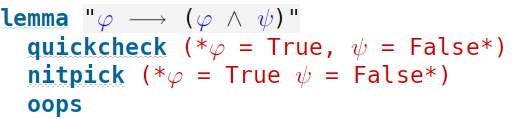
\includegraphics[width=0.5\linewidth]{Isabelle-counter}
    \caption{Example of code in Isabelle testing Nitpick and Quickcheck.}
    \label{img:isabelle-counter}
\end{figure}

\subsection{Lean}
\label{chap:lean}
Lean is a functional programming language that can be used as an interactive theorem prover~\cite{programming}. The structure of the proofs in this tool is very similar to the one presented in~\ref{chap:prop-deduction}, where it is possible to use rules defined in \gls{ND}, in contrast to Isabelle/HOL. Figure \ref{img:lean_example} shows an example of a proof in \gls{ND} using Lean's style, while Figure \ref{tab:lean_example} presents its representation in tree form.

\begin{figure}[htbp]
    \centering
    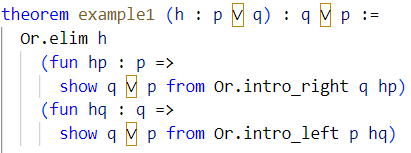
\includegraphics[width=0.5\linewidth]{Lean_example}
    \caption{Example of code in Lean proving \(\{p \lor q\} \models q \lor p \).}
    \label{img:lean_example}
\end{figure}

\begin{figure}[h!]
    \centering
        \[
            \frac{ {\displaystyle {p \lor q}^1 
            \quad \quad \displaystyle \frac{\displaystyle p^2}{q \lor p \strut} (\lor I_l) \strut}
            \quad \quad \displaystyle \frac{\displaystyle q^3}{q \lor p \strut} (\lor I_r) \strut}
            {\displaystyle q \lor p \strut} \quad (\vee E, 2, 3)
          \]
          \caption{Example of a deduction tree proving \(\{p \lor q\} \models q \lor p \).}
          \label{tab:lean_example}
      \end{figure}

Lean also has a tool to automate proofs called Aesop~\cite{leanprovercommunity_2021_github}. Unlike Isabelle/HOL, Aesop can provide a step-by-step proof, but not in the format presented above. The generated proof uses different tactics that are generally not easy to directly map to \gls{ND} rules. However, Aesop allows users to define their own rules/tactics to help with automation. It is possible to restrict the domain of the rules used in the automation process. Perhaps by defining the set of all \gls{ND} rules, we could achieve the desired output, enabling the generation of proofs using only valid rules. If we successfully accomplish this, we will have a reliable method for implementing our feedback. Another interesting feature of Aesop is that it allows the user to use part of their proof to generate the rest of it when possible.




